% Created 2018-07-11 Wed 15:29
% Intended LaTeX compiler: pdflatex
\documentclass[11pt]{article}
\usepackage[utf8]{inputenc}
\usepackage[T1]{fontenc}
\usepackage{graphicx}
\usepackage{grffile}
\usepackage{longtable}
\usepackage{wrapfig}
\usepackage{rotating}
\usepackage[normalem]{ulem}
\usepackage{amsmath}
\usepackage{textcomp}
\usepackage{amssymb}
\usepackage{capt-of}
\usepackage{hyperref}
\date{\today}
\title{}
\hypersetup{
 pdfauthor={},
 pdftitle={},
 pdfkeywords={},
 pdfsubject={},
 pdfcreator={Emacs 26.0.91 (Org mode 9.1.13)}, 
 pdflang={English}}
\begin{document}

\tableofcontents

\section{Personalmanagement}
\label{sec:orge0e7ce5}
\subsection{Personal \& Wettbewerbsfähigkeit}
\label{sec:org0dc8524}
Das Ausgangsproblem dreht sich um die optimale Ergiebigkeit menschlicher Arbeitsleistung (Gutenberg).

Kategorien/Ebenen personalwirtschaftlichen Handelns:
\begin{itemize}
\item Zielebene = Verfügbarkeit \& Wirksamkeit von Personal
\item Instrumentenebene = Selektion personalwirtschaftlicher Maßnahmen (Instrumente/Ergebnisse) und ihre Wirkungen (intendiert / nicht intendiert)
\item Erfolgsebene = Management der Humanressourcen und Unternehmenserfolg
\end{itemize}

\subsubsection{Personalwirtschaftliches Handeln}
\label{sec:org8416789}
Geht man davon aus, dass ein bestimmter personalwirtschaftlicher Zweck prinzipiell durch verschiedene Handlungen erreicht werden kann, dass außerdem eine bestimmte Handlung prinzipiell verschiedenen personalwirtschaftlichen Zwecken dienen kann und dass schließlich Handlungen auch 'nicht-bezweckte'(nicht-intendierte) Wirkungen hervorrufen können, so werden \emph{Wahlprobleme} sichtbar, die sich mit Hilfe von elementaren \emph{Kategorien} charakterisieren lassen.

Personalwirtschaftl. Probleme entstehen, wenn Unternehmer andere Personen zur Deckung des Arbeitskräftebedarfs in einer Weise in Dienst stellen dass diese bestimmte Dispositionsbefugnisse über ihre Arbeitskraft gegen eine festgelegte Vergütung direkt oder indirekt auf den Unternehmer übertragen.

Prolemkategorien:
\begin{itemize}
\item Herstellung \& Sicherung der Verfügbarkeit \emph{über} Personal (\textbf{Disponibilität})
\begin{itemize}
\item menschliche Arbeitskraft ist ein knappes "Gut"
\item menschliche Arbeitskraft wird in versch Qualität nachgefragt \& angeboten
\item der Bedarf des Betriebes an Personal verändert sich quantitativ und/oder strukturell
\item eine zu einem bestimmten Zeitpunkt gegebene Ausstattung eines Betriebes mit Personal unterliegt im Zeitablauf quantitativen und/oder strukturellen Veränderungen, die nicht durch betriebliche Dispositionen induziert werden
\end{itemize}
\item Herstellung \& Sicherung der Verfügbarkeit \emph{des} Personal (\textbf{Funktionalität})
\begin{itemize}
\item Ansprüche an das Verhalten des Personals sind je nach Situation bzgl ihres konkreten Inhalts und ihres relativen Gewichts unterschiedlich
\item Personal wird idR aufgrund von Selbstdarstellung, Fremdeinschätzung \& Verhaltensstichproben ausgewählt, deren Aussageberich beschränkt und deren Aussagekraft häufig gering sind
\item die Annahme, das sich die Arbeitskräfte mit den Verhaltensansprüchen der Organisation identifizieren, trifft im Regelfall weder für die Verhaltensansprüche noch für alle Angehörigen eines Betriebens in gleicher Weise zu
\item die Erfüllung von Verhaltensansprüchen muss den Mitarbeitern möglich sein
\end{itemize}
\end{itemize}

\subsubsection{Instrumentenebende personalwirtschaftlichen Handelns}
\label{sec:org9702ca9}
\begin{figure}[htbp]
\centering
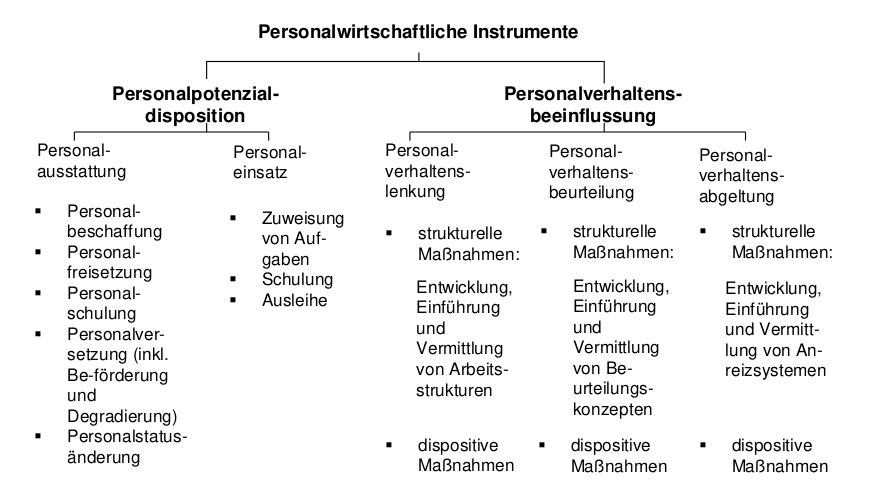
\includegraphics[width=250px]{./pictures/persinstr.png}
\caption{Instrumentenebene personalwirtschaftlichen Handelns}
\end{figure} 

\subsubsection{Zielebene personalwirtschaftlichen Handelns}
\label{sec:org3730c41}
\begin{itemize}
\item Individuelle Schutzreche
\begin{itemize}
\item Schutz des Arbeitsverhältnisses (zB Kündigungsschutz)
\item Schutz der Gesundheit (zB Emissionschutz, Arbeitsschutz)
\item besondere Schutzrechte (zB für gefährdete Mitarbeitergruppen)
\end{itemize}
\item Arbeitsrechtliche Mitbestimmung
\begin{itemize}
\item Beteiligung bei sozialen \& personellen Entscheidungen
\item Informations-, Beratungs-, Mitwirkungs- und Mitbestimmungsrechte
\item Interessenvertretung durch Betriebsrat, Jugendvertretung, Wirtschaftsausschuss oä
\end{itemize}
\item Unternehmerische Mitbestimmung
\begin{itemize}
\item Mitwirkungsrechte bei unternehmerischen Entscheidungen
\end{itemize}
\end{itemize}

\subsubsection{Erfolgsebene personalwirtschaftlichen Handelns}
\label{sec:orgdc31938}
\begin{figure}[htbp]
\centering
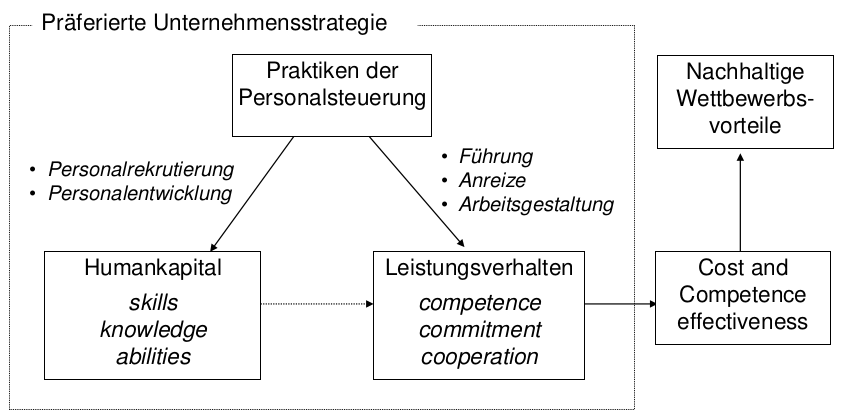
\includegraphics[width=250px]{./pictures/perserfolg.png}
\caption{Management der Humanressourcen \& Unternehmenserfolg}
\end{figure} 
\subsubsection{Elementarkategorien personalwirtsch Handelns (Zusammenfassung)}
\label{sec:org7cff8dd}
\begin{figure}[htbp]
\centering
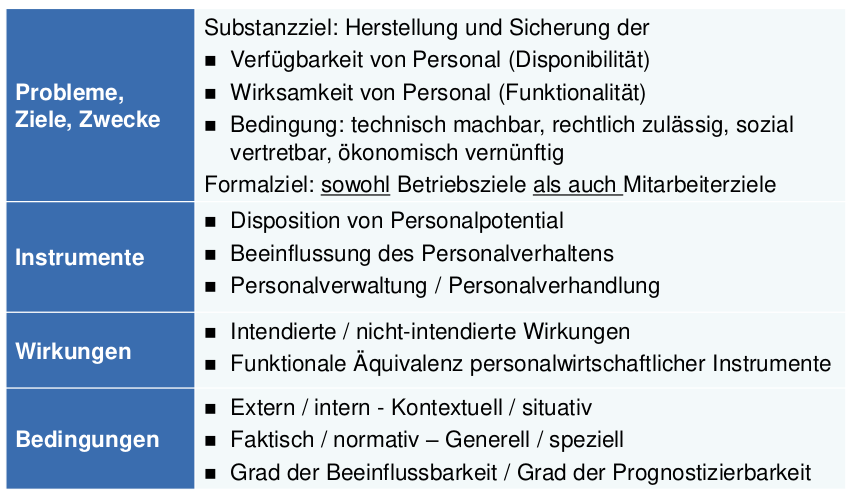
\includegraphics[width=250px]{./pictures/perskateg.png}
\caption{Instrumentenebene personalwirtschaftlichen Handelns}
\end{figure} 

\subsection{Disposition des Personalpotentials}
\label{sec:orgceca750}
\subsubsection{Personalbedarf}
\label{sec:orgf4533a2}
Der \emph{Personalbedarf} einer Organisation umfasst - nach geforderten Qualifikationsstrukturen - gruppiert die Gesamtheit, die zur Wahrnehmung aller dispositiven \& exekutiven Aufgaben in allen Bereichen und auf allen Ebenen einer Organisation benötigt werden.

Primärdeterminanten:
\begin{itemize}
\item periodenbezogenes Leistungsprogramm eines Betriebes
\item Arbeitszeitbedarf pro Leistungseinheit (Arbeitskoeffizient) bzw pro zu bedienender Bestandseinheit (Besetzungskoeffizient)
\item verfügbare Arbeitszeit der Arbeitskraft pro Periode
\end{itemize}

Sekundärdeterminanten:
\begin{itemize}
\item Angebots-/Nachfrageverhältnis, Technologie (zB Automatisierungsgrad), Grad der Arbeitsteilung
\item Anforderungsprofile/Stellenbeschreibungen
\end{itemize}

Verfügbarkeit des Personals \(\rightarrow\) Dispositionsabhängigkeit der Bestimmung \& Deckung des Personalbedarfs
\subsubsection{Personalrekrutierung und -auswahl}
\label{sec:org93870d3}
Anwerbung
\begin{itemize}
\item Zweck = Herstellung von Kontakten zu potentiellen Bewerbern, Personalmarketing (Arbeitgeberimage)
\item Funktionen = Information, Motivation, Vorselektion
\item Methoden = passiv, aktiv (zB Stellenanzerigen, elektr. Jobbörsen)
\end{itemize}

Auswahl
\begin{itemize}
\item Zweck = Identifikation der Eignung von Bewerbern für eine zu besetzende Stelle/Position, Screening-Strategie
\item Phasen = Vorauswahl, Auswahl
\item Methoden = Eignungstest, Assessment Center, Auswahlgespräch
\end{itemize}

Einstellung
\begin{itemize}
\item Zweck = Vereinbarungen zum Arbeitsverhältnis und zur Arbeitsleistung
\item Inhalt = Kompetenzabgrenzung, Arbeitsbedingungen, berufliche Entwicklungsperspektiven
\item impliziter Vertrag =  Vereinbarung von Rechten \& Pflichten auf der Basis stillschweigender Übereinkünfte
\end{itemize}

Eingliederung
\begin{itemize}
\item Zweck = Einführung des Mitarbeiters in das Arbeits-/Aufgabenfeld
\item Inhalt = bereichsübergreifende, fachliche, soziale Eingliederung
\end{itemize}

Berufsbozgenes Integritätsprofil als Profil/Einschätzung der Eignung. Baumquerschnittdiagramm mit verschiedenen Charaktereigenschaften wie Gelassenheit, Vertrauen, Zuverlässigkeit, Verzicht auf Rechtfertigung etc.

\textbf{Einstellungsinterviews}\\
unstrukturiertes Interview:
\begin{itemize}
\item Annahmen über Menschenkenntnis
\item Unterstützung von Stereotypen
\item Annahmen über ideale Persönlichkeit
\item hohe Wirkung von non-verbalem Verhalten
\end{itemize}

strukturiertes Interview:
\begin{itemize}
\item anforderungsbezogene Gestaltung
\item Interviewverlauf und Fragenabfolge sind strukturiert
\item Verwendung validierter/bewährter Merkmale
\item Information \& Entscheidung sind getrennt (Beratungszeit)
\item mehrere unabhängige \& kompetente Beurteiler sind beteiligt
\end{itemize}


\begin{figure}[htbp]
\centering
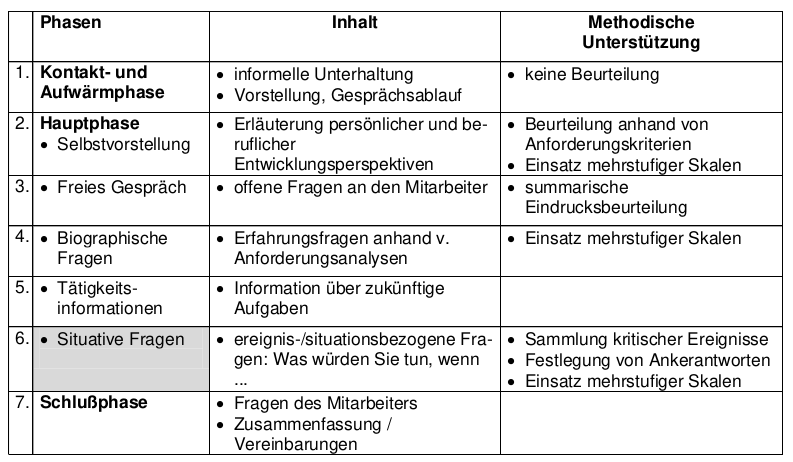
\includegraphics[width=250px]{./pictures/persint.png}
\caption{Multimodales Interview}
\end{figure} 
\subsubsection{Einsatz \& Disposition des Personals}
\label{sec:orgc04aacb}
Einsatz von Personal
\begin{itemize}
\item Zweck =  Übertragung von Aufgaben oder Stellen an die vorhandenen/verfügbaren Arbeitskräfte
\item Methode = Zuordnung von Anforderungsprofilen und Fähigkeitsprofilen auf der Basis von Mindestwerten (Cut-Off Methode) oder (gewichteten) Ähnlichkeiten (Profilvergleichsmethode)
\end{itemize}

Segmentierung des Personals
\begin{itemize}
\item Differenzierung der Verfügbarkeit des Personals nach spezifischen Beschäftigungs-, Arbeits- und Entgeltbedingungen
\item Stammbelegschaft = internes Arbeitsmarktsegment
\item Randbelegschaft = externes Arbeitsmarktsegment (Manövriermasse für quantitative Anpassungen des Personalbestands)
\end{itemize}

Personalplanung als Disposition \(\rightarrow\) die Aufgabe der Personalplanung ist es, den Personalbedarf, den Personaleinsatz und die Personalaustattung - unter Beachtung der für den Personalsektor geltenden Restriktionen - optimal im Sinne der betrieblichen Ziele aufeinander abzustimmen
\subsubsection{Personalentwicklung}
\label{sec:orga62e0c5}
\begin{figure}[htbp]
\centering
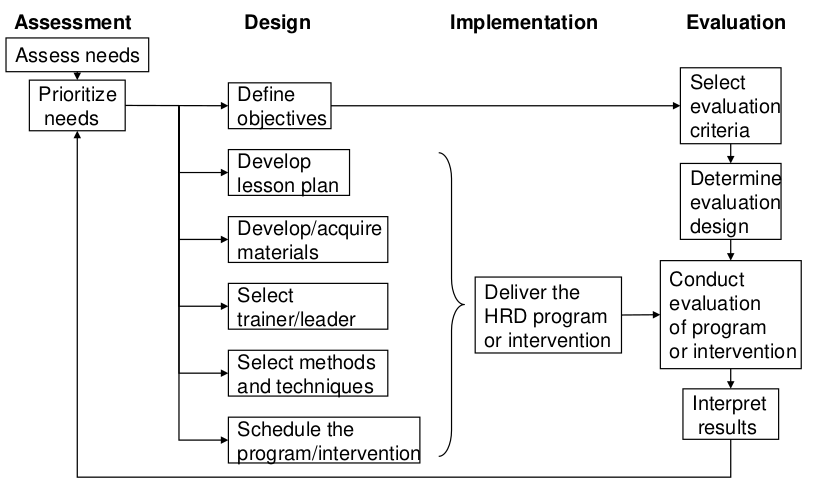
\includegraphics[width=250px]{./pictures/persgruent.png}
\caption{Grundmodell der Personalentwicklung}
\end{figure} 

Beeinflussung des Personalverhaltens nicht klausurrelevant!

\textbf{Ansprüche als Kriterium der Verhaltensbeeinflussung}:

Beeinflussung des Personalverhaltens
\begin{itemize}
\item Zweck = Durchsetzung von Ansprüchen der Organisation an das Personalverhalten (Verhaltenserwartung)
\item Inhalt = Aufforderung, sich in einer bestimmten Art \& Weise zu Verhalten (Anspruchskonformität des Verhaltens)
\end{itemize}

Inhaltsklassen organisationaler Ansprüche
\begin{itemize}
\item Funktional = Verhaltenserwartungen, die sich auf die Arbeitsaufgaben und die Arbeitsergebniise beziehen (\(\rightarrow\) Qualitätsansprüche, Gestaltungsansprüche)
\item Extrafunktional = Verhaltenserwartungen, die sich insbes auf das Sozialverhalten beziehen (\(\rightarrow\) Höflichkeit, Ehrlichkeit, Pünktlichkeit)
\item Situationsabhängigkeit von Verhaltenserwartungen
\end{itemize}

Maßnahmen zur Verhaltensbeeinflussung
\begin{itemize}
\item Verhaltenslenkung
\item Verhaltensbeurteilung
\item Verhaltensabgeltung
\end{itemize}


\textbf{Strukturelle Maßnahmen zur Beeinflussung des Personalverhaltens}
\begin{itemize}
\item strukturelle Maßnahmen = Arbeitsstruktur, Beurteilung, Anreize
\item Entlohnung als Anreiz
\end{itemize}
\begin{figure}[htbp]
\centering
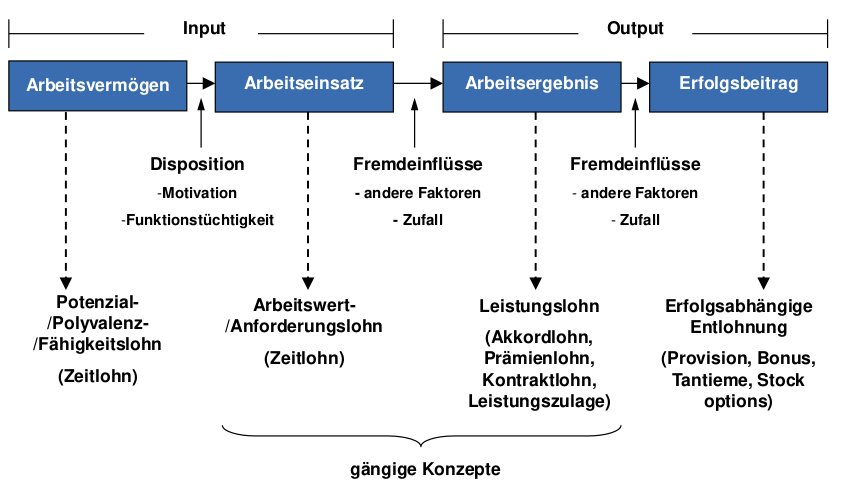
\includegraphics[width=250px]{./pictures/persentl.png}
\caption{Bemessungsgrundlagen \& Formen der Entlohnung}
\end{figure} 



\textbf{Dispositive Maßnahmen zur Beeinflussung des Personalverhaltens}
\begin{itemize}
\item dispositive Maßnahmen = Beeinflussung durch situationsabhängies Führungsverhalten
\item Führungskonzept, Situation und Führungserfolg
\begin{itemize}
\item Kontingenzmodell der Führung nach Fiedler
\item Situative Führungstheorie nach Hersey/Blanchard
\end{itemize}
\end{itemize}

III\(_{\text{Personalmanagement}}\)\(_{\text{3.pdf}}\) F.13 Zsmfassung
\end{document}
